\chapter{सजीवों की छँटाई}\label{ch:g3:sorting-living-things}

मिले-जुले बटनों का डिब्बा मेज़ पर उँडेलो और तुम्हारे हाथ अपने आप छाँटने
लगते हैं: बड़े बड़ों के साथ, लाल लालों के साथ, चार छेद वालों के साथ
चार छेद वाले। भृंगों, \omterm{prop:g3:sorting-living-things:groups}{पक्षियों}, फ़र्नों और \omterm{prop:g3:sorting-living-things:groups}{मछलियों} से भरी जीवित दुनिया
के सामने प्रकृतिविदों को भी यही ललक हुई --- और सजीवों की सावधानी से
की गई छँटाई \omterm{def:g1:living-or-not:living}{जीवविज्ञान} के सबसे ताक़तवर विचारों में से एक निकली।

\section{छाँटने के लिए एक नियम चाहिए}

\begin{definition}[छँटाई और मानदंड]\label{def:g3:sorting-living-things:criterion}
किसी संग्रह को \emph{छाँटना}\index{छँटाई} यानी उन चीज़ों को साथ रखना जो
साथ जाती हैं। \emph{मानदंड}\index{मानदंड} वह नियम है जिससे छँटाई की
जाती है --- ``छह \omterm{def:g1:my-body:parts}{टाँगें} हैं'', ``\omterm{def:g1:animals-around-us:covering}{पंख} हैं''। सजीवों के लिए अच्छा मानदंड
शरीर की वह ख़ासियत है जिसका तुम \emph{प्रेक्षण} कर सको: यानी जो उस \omterm{def:g1:animals-around-us:animal}{जंतु}
या \omterm{def:g1:plants-around-us:plant}{पौधे} के \emph{पास है}, न कि उसकी रहने की जगह या वह जो कर रहा हो।
\end{definition}

\begin{example}[एक ही जंतुओं की दो छँटाइयाँ]\label{ex:g3:sorting-living-things:two}
बिल्ली, बत्तख़, ट्राउट और गुबरैला लो। ``पानी के पास रहता है'' से छाँटो:
बत्तख़ और ट्राउट साथ। ``\omterm{def:g1:animals-around-us:covering}{पंख} हैं'' से छाँटो: बत्तख़ अकेली रह जाती है।
दोनों छँटाइयाँ हैं --- पर दूसरी ही \omterm{def:g1:animals-around-us:animal}{जंतु} के अपने शरीर का इस्तेमाल करती
है, और जीवविज्ञानी इसी पर भरोसा करते हैं: \omterm{def:g1:animals-around-us:animal}{जंतु} घर बदल सकता है, पर वह
अपने \omterm{def:g1:animals-around-us:covering}{पंखों} को \omterm{def:g1:animals-around-us:covering}{शल्कों} से नहीं बदल सकता।
\end{example}

\begin{remark}[घर या मेनू से क्यों न छाँटें?]\label{rem:g3:sorting-living-things:why}
\omterm{def:g2:where-animals-live:habitat}{आवास} और मेनू मौसम और संयोग के साथ बदलते हैं ---
\cref{ch:g2:what-animals-eat} की कलचिड़ी केंचुओं से जामुनों पर आ जाती
है और इससे कोई दूसरा \omterm{def:g1:animals-around-us:animal}{जंतु} नहीं बन जाती। शरीर की ख़ासियतें टिकी रहती
हैं। इसीलिए छँटाई के नियम के रूप में ``इसके पास क्या है'' ``यह क्या
करता है'' से बेहतर है।
\end{remark}

\section{जंतुओं के बड़े समूह}

\begin{proposition}[कुछ बड़े समूह]\label{prop:g3:sorting-living-things:groups}
शरीर की ख़ासियतों से की गई छँटाई \omterm{def:g1:animals-around-us:animal}{जंतुओं} को बड़े समूहों में इकट्ठा कर
देती है, जिनमें ये भी हैं:
\begin{itemize}
  \item \emph{कीट}\index{कीट}: छह \omterm{def:g1:my-body:parts}{टाँगें}, तीन हिस्सों वाला शरीर ---
        चींटी, गुबरैला, मधुमक्खी, तितली;
  \item \emph{मछलियाँ}\index{मछली}: मीन-पंख और \omterm{def:g1:animals-around-us:covering}{शल्क}, पूरा जीवन पानी
        में --- ट्राउट, सुनहरी मछली;
  \item \emph{पक्षी}\index{पक्षी}: \omterm{def:g1:animals-around-us:covering}{पंख}, डैने और चोंच --- बत्तख़,
        कलचिड़ी, शुतुरमुर्ग़;
  \item \emph{स्तनधारी}\index{स्तनधारी}: \omterm{def:g1:animals-around-us:covering}{रोम} या बाल, और ऐसी माँएँ जो
        अपने बच्चों को \omterm{def:g2:animals-grow-up:born}{दूध} पिलाती हैं --- बिल्ली, गाय, चमगादड़, ह्वेल
        --- और मनुष्य;
  \item \emph{उभयचर}\index{उभयचर}: नम \omterm{def:g1:the-five-senses:sense}{त्वचा}, पानी में दिए \omterm{def:g2:animals-grow-up:born}{अंडे},
        \omterm{ex:g2:animals-grow-up:frog}{टैडपोल} वाला बचपन --- मेंढक, न्यूट।
\end{itemize}
\end{proposition}
\admitted

\begin{omfigure}
\begin{tikzpicture}
  \foreach \x/\name/\feat in {
      0/कीट/{6 टाँगें},
      2.95/मछलियाँ/{मीन-पंख, शल्क},
      5.9/पक्षी/{पंख, चोंच},
      8.85/स्तनधारी/{रोम, दूध},
      11.8/उभयचर/{नम त्वचा}} {
    \draw[thick, omDef, fill=omDef!6, rounded corners=5pt]
      (\x,0) rectangle ({\x+2.8},1.7);
    \node[font=\small\bfseries, text height=1.6ex, text depth=0.4ex]
      at ({\x+1.4},1.3) {\name};
    \node[font=\small, text height=1.6ex, text depth=0.4ex]
      at ({\x+1.4},0.6) {\feat};
  }
\end{tikzpicture}

{\small पाँच बड़े समूह, हर एक का नाम इसी पर कि उसके सदस्यों के पास
क्या \emph{है}।}
\end{omfigure}

\begin{example}[चौंकाने वाले, ठीक से सुलझे]\label{ex:g3:sorting-living-things:surprises}
\omterm{def:g3:sorting-living-things:criterion}{मानदंड} हमें आलसी अंदाज़ों से बचाते हैं। चमगादड़ \omterm{prop:g3:sorting-living-things:groups}{पक्षी} की तरह उड़ता है
--- पर उसके \omterm{def:g1:animals-around-us:covering}{रोम} हैं, \omterm{def:g1:animals-around-us:covering}{पंख} नहीं, और वह अपने बच्चों को \omterm{def:g2:animals-grow-up:born}{दूध} पिलाता है:
यानी \omterm{prop:g3:sorting-living-things:groups}{स्तनधारी}। ह्वेल मछली की तरह तैरती है --- उसके \omterm{def:g1:animals-around-us:covering}{रोम} लगभग ग़ायब हैं,
पर वह अपने बच्चे को \omterm{def:g2:animals-grow-up:born}{दूध} पिलाती है और उसके \omterm{def:g1:animals-around-us:covering}{शल्क} नहीं होते: यह भी
\omterm{prop:g3:sorting-living-things:groups}{स्तनधारी}। शुतुरमुर्ग़ उड़ ही नहीं सकता, फिर भी \omterm{def:g1:animals-around-us:covering}{पंख} और चोंच कहते हैं:
\omterm{prop:g3:sorting-living-things:groups}{पक्षी}। फ़ैसला \omterm{def:g3:sorting-living-things:criterion}{मानदंड} करता है, पहली नज़र का असर नहीं।
\end{example}

\begin{omfigure}
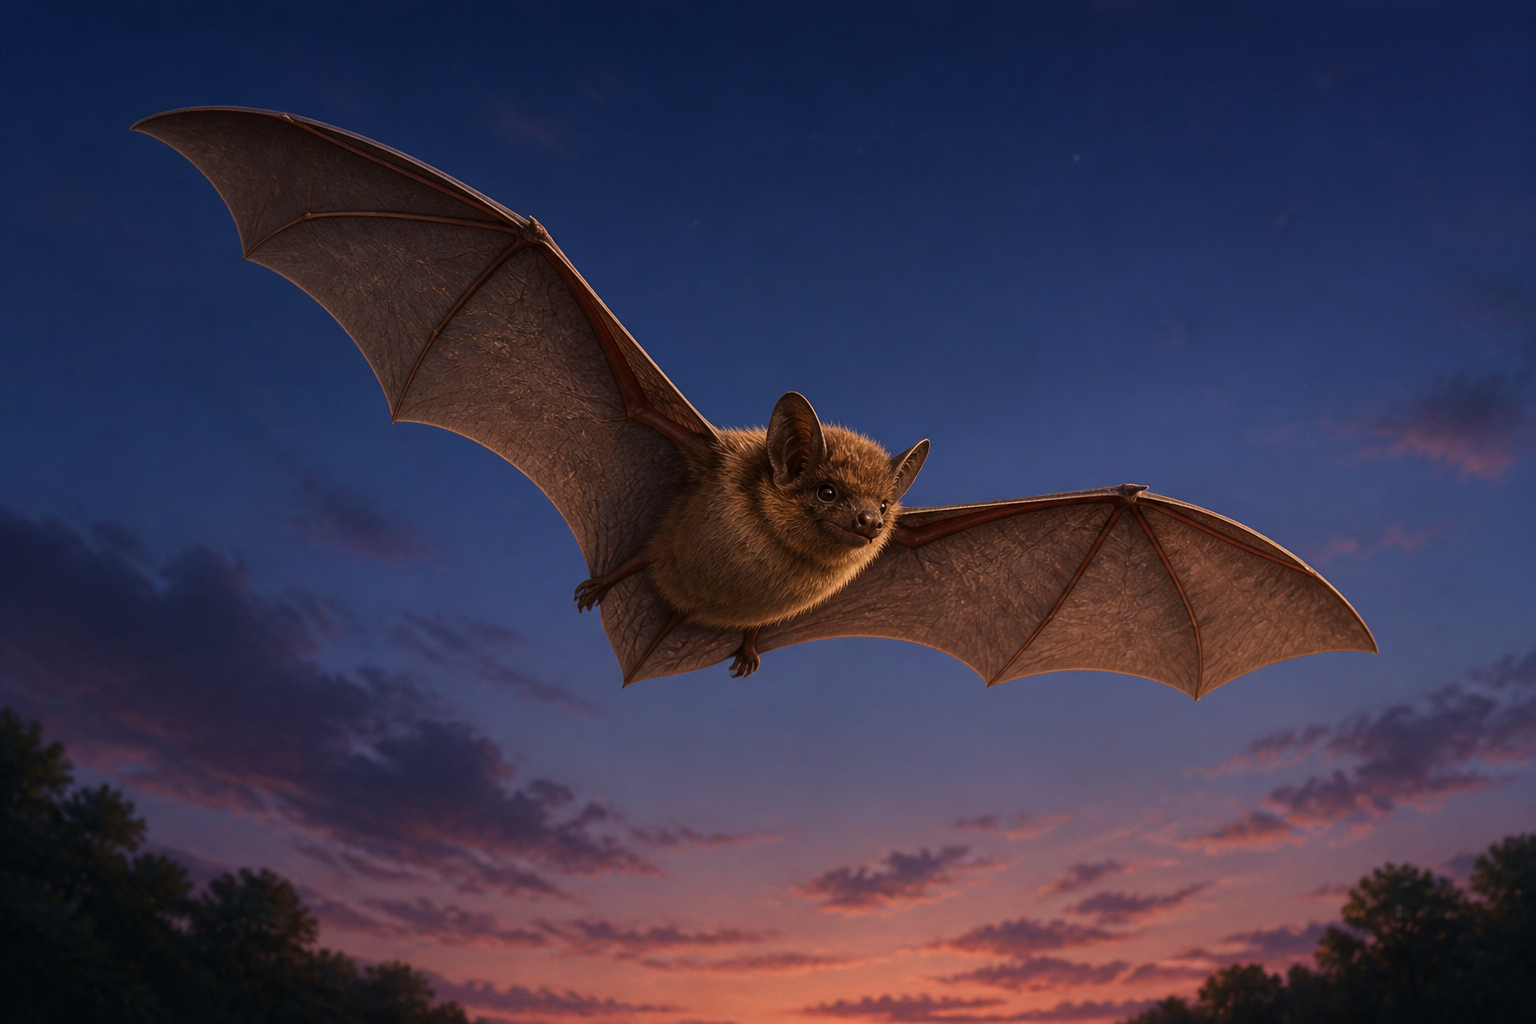
\includegraphics[width=0.6\linewidth]{images/book1/ai/g3-sort-bat.png}

{\small वह \omterm{prop:g3:sorting-living-things:groups}{पक्षी} की तरह उड़ता है --- और नंगे डैनों पर \omterm{def:g1:animals-around-us:covering}{रोम} पहनता है:
चमगादड़, यानी पहली नज़र के बजाय ख़ासियतों से छाँटने की सबसे मशहूर
कसौटी।}
\end{omfigure}

\begin{method}[अनजान जंतु की छँटाई]\label{met:g3:sorting-living-things:sort}
\begin{enumerate}
  \item शरीर का प्रेक्षण करो: \omterm{def:g1:the-five-senses:sense}{त्वचा}, \omterm{def:g1:animals-around-us:covering}{रोम}, \omterm{def:g1:animals-around-us:covering}{पंख} या \omterm{def:g1:animals-around-us:covering}{शल्क}? कितनी \omterm{def:g1:my-body:parts}{टाँगें}?
        डैने? चोंच?
  \item हो सके तो बच्चों के बारे में पूछो: \omterm{def:g2:animals-grow-up:born}{दूध}? \omterm{def:g2:animals-grow-up:born}{अंडे}? \omterm{ex:g2:animals-grow-up:frog}{टैडपोल} वाली
        अवस्था?
  \item \cref{prop:g3:sorting-living-things:groups} के समूहों से
        तुलना करो और \omterm{def:g1:animals-around-us:animal}{जंतु} को वहाँ रखो जहाँ उसकी \emph{ख़ासियतें}
        बैठती हैं;
  \item अगर पहली नज़र का असर (``यह तो उड़ता है!'') किसी ख़ासियत
        (``इसके \omterm{def:g1:animals-around-us:covering}{रोम} हैं'') से न मिले, तो ख़ासियत पर भरोसा करो।
\end{enumerate}
\end{method}

\section{पौधों की भी छँटाई होती है}

\begin{proposition}[पौधों की छँटाई]\label{prop:g3:sorting-living-things:plants}
\omterm{def:g1:plants-around-us:plant}{पौधों} को भी \omterm{def:g1:animals-around-us:animal}{जंतुओं} की तरह उनकी ख़ासियतों से छाँटा जाता है। काम के
\omterm{def:g3:sorting-living-things:criterion}{मानदंड}: क्या उसमें \emph{\omterm{def:g1:plants-around-us:parts}{फूल}} और \omterm{def:g2:from-seed-to-plant:seed}{बीज} बनते हैं (गुलबहार, चेस्टनट) या
कभी नहीं बनते (फ़र्न, मॉस)? क्या उसका \omterm{def:g1:plants-around-us:parts}{डंठल} मुलायम और हरा है, या
\emph{\omterm{def:g1:plants-around-us:tree}{पेड़}} के तने जैसा लकड़ी का? क्या \omterm{def:g1:plants-around-us:parts}{पत्तियाँ} चौड़ी हैं, या चीड़ की
तरह सुइयाँ?
\end{proposition}
\admitted

\begin{example}[पार्क के तीन कोने]\label{ex:g3:sorting-living-things:park}
एक ही पार्क में: गुलाब की झाड़ी --- \omterm{def:g1:plants-around-us:parts}{फूल}, लकड़ी के \omterm{def:g1:plants-around-us:parts}{डंठल}; उत्तर की दीवार
पर मॉस --- कभी कोई \omterm{def:g1:plants-around-us:parts}{फूल} नहीं, कोई असली \omterm{def:g1:plants-around-us:parts}{डंठल} भी नहीं; और चीड़ --- सुइयों
और शंकुओं वाला \omterm{def:g1:plants-around-us:tree}{पेड़}। तीन \omterm{def:g1:plants-around-us:plant}{पौधे}, एक ही \omterm{def:g3:sorting-living-things:criterion}{मानदंडों} के तीन अलग-अलग उत्तर।
\end{example}

\begin{remark}[छँटाई विज्ञान का पहला क़दम है]\label{rem:g3:sorting-living-things:science}
ठीक से छाँटे गए समूह लोगों को बेहतर सवाल पूछने देते हैं: जो कुछ आम तौर
पर \omterm{prop:g3:sorting-living-things:groups}{कीटों} के बारे में सच है --- छह \omterm{def:g1:my-body:parts}{टाँगें}, तीन हिस्सों वाला शरीर, अकसर
डैने --- वह एक ही झटके में लाखों प्रजातियों के बारे में जान लिया जाता
है। आगे के अध्याय छँटाई को सारे सजीवों के कुल-वृक्ष में बदल देंगे ---
फ़िलहाल जो दिख सके, उसी से छाँटना सीखो।
\end{remark}

\section{अभ्यास}

\begin{exercise}[$\star$]\label{exo:g3:sorting-living-things:1}
\omterm{def:g3:sorting-living-things:criterion}{मानदंड} क्या है? \omterm{def:g1:animals-around-us:animal}{जंतुओं} की छँटाई के लिए एक अच्छा \omterm{def:g3:sorting-living-things:criterion}{मानदंड} बताओ, और एक ऐसा
जिससे जीवविज्ञानी बचते हैं।
\end{exercise}

\begin{exercise}[$\star$]\label{exo:g3:sorting-living-things:2}
हर समूह को परिभाषित करने वाली ख़ासियत (या ख़ासियतें) बताओ: \omterm{prop:g3:sorting-living-things:groups}{कीट},
\omterm{prop:g3:sorting-living-things:groups}{मछलियाँ}, \omterm{prop:g3:sorting-living-things:groups}{पक्षी}, \omterm{prop:g3:sorting-living-things:groups}{स्तनधारी}।
\end{exercise}

\begin{exercise}[$\star$]\label{exo:g3:sorting-living-things:3}
हर \omterm{def:g1:animals-around-us:animal}{जंतु} को उसके समूह में रखो: मधुमक्खी, सुनहरी मछली, शुतुरमुर्ग़, गाय,
मेंढक।
\end{exercise}

\begin{exercise}[$\star$]\label{exo:g3:sorting-living-things:4}
चमगादड़ उड़ता है। फिर वह \omterm{prop:g3:sorting-living-things:groups}{पक्षी} नहीं, \omterm{prop:g3:sorting-living-things:groups}{स्तनधारी} क्यों है? कौन-सी
ख़ासियतें फ़ैसला करती हैं?
\end{exercise}

\begin{exercise}[$\star$]\label{exo:g3:sorting-living-things:5}
ह्वेल समुद्र में रहती है। फिर वह मछली क्यों नहीं है? कौन-सी ख़ासियतें
फ़ैसला करती हैं?
\end{exercise}

\begin{exercise}[$\star$]\label{exo:g3:sorting-living-things:6}
मकड़ी की आठ \omterm{def:g1:my-body:parts}{टाँगें} होती हैं। क्या वह \omterm{prop:g3:sorting-living-things:groups}{कीट} हो सकती है? \omterm{def:g3:sorting-living-things:criterion}{मानदंड} क्या उत्तर
देता है?
\end{exercise}

\begin{exercise}[$\star$]\label{exo:g3:sorting-living-things:7}
\cref{prop:g3:sorting-living-things:plants} के \omterm{def:g3:sorting-living-things:criterion}{मानदंडों} से इन \omterm{def:g1:plants-around-us:plant}{पौधों} को
छाँटो: गुलबहार, मॉस, चीड़, गुलाब की झाड़ी।
\end{exercise}

\begin{exercise}[$\star$]\label{exo:g3:sorting-living-things:8}
करके देखो: अपनी गली या बग़ीचे के \omterm{def:g1:animals-around-us:animal}{जंतुओं} को --- जितने एक सैर में दिख
जाएँ --- इस अध्याय के समूहों में छाँटो। संख्या में कौन-सा समूह जीतता
है?
\end{exercise}

\begin{exercise}[$\star\star$]\label{exo:g3:sorting-living-things:9}
लीना \omterm{def:g1:animals-around-us:animal}{जंतुओं} को ``पालतू'' और ``जंगली \omterm{def:g1:animals-around-us:animal}{जंतु}'' में छाँटती है। उसकी सहेली
उन्हीं \omterm{def:g1:animals-around-us:animal}{जंतुओं} को ``\omterm{prop:g3:sorting-living-things:groups}{स्तनधारी}'' और ``\omterm{prop:g3:sorting-living-things:groups}{पक्षी}'' में छाँटती है। किसकी छँटाई
जीवविज्ञानी वाली है, और क्यों?
\cref{rem:g3:sorting-living-things:why} का इस्तेमाल करो।
\end{exercise}

\begin{exercise}[$\star\star$]\label{exo:g3:sorting-living-things:10}
पेंग्विन बहुत बढ़िया तैरता है, उड़ नहीं सकता, और उस पर चमकीली टाइलों
जैसा कुछ ढका रहता है। एक प्रकृतिविद ग़ौर से देखता है: वे ``टाइलें''
कसकर जमे हुए \omterm{def:g1:animals-around-us:covering}{पंख} हैं, और एक चोंच भी है। पेंग्विन पर
\cref{met:g3:sorting-living-things:sort} चरण दर चरण चलाओ।
\end{exercise}
